\documentclass{article}

\usepackage{graphicx}
\usepackage{setspace}
\usepackage{listings}
\usepackage{color}
\usepackage{circuitikz}
\usepackage{float}

% Set margins to 0.5inch
\usepackage[margin=1in]{geometry}


\title{ECE 210 - Combinational Logic Design \\ Lab 3}
\date{2018-11-07}
\author{Radomir Wasowski \\ wasowski@ualberta.ca
        \and David Lenfesty \\ lenfesty@ualberta.ca}

\setcounter{tocdepth}{2} % Show subsections

\definecolor{dkgreen}{rgb}{0,0.6,0}
\definecolor{gray}{rgb}{0.5,0.5,0.5}
\definecolor{mauve}{rgb}{0.58,0,0.82}

\lstset{basicstyle=\small,
        keywordstyle=\color{mauve},
        identifierstyle=\color{dkgreen},
        stringstyle=\color{gray},
        numbers=left
        }

\begin{document}

\pagenumbering{gobble}
\doublespacing
\maketitle
\newpage

\singlespacing

\section{Abstract}

Display technology allows designers to display changing and important information to users.
By using logic gates to implement a 7-segment display that can directly output the value of a sensor,
an effective user interface can be built.

\section{Introduction}

In this lab we were tasked with designing VHDL circuits that were able to update a 7-segment display
in order to display hexadecimal digits.
In parts 1 \& 2, we were asked to do this using structural and behavioural logic, respectively.
Parts 3 \& 4 tasked us to use this display to in order to count from 0x0 to 0xF, on one or two seperate displays.

\section{Design}

\paragraph{Part 1:}

Because many characters, when displayed on a 7-segment display, share common elements,
it is relatively trivial to combine logic signals using minterms or maxterms.
Using Karnaugh maps of each different letter based on the 4-bit input, a series of logical outputs
were found, which were then connected to the appropriate display segments.
Because of this, the number of discrete logic elements could be vastly reduced.
Once these signals were found, they were transcribed into a VHDL file,
to be uploaded to an FPGA for testing.

\paragraph{Part 2:}

Instead of defining all of the logic gates manually, VHDL also supports
behavioural programming.
This style is different in that the synthesizer will decide how to implement
the code in logic, instead of the programmer doing the heavy lifting.
By utilizing a case statement, writing the program could be made easier,
as the designer does not have to worry about exactly how the logic should work.
However, this method does take some of the control over how the circuit operates
away from the designer.

\paragraph{Part 3:}

By using one of the inbuilt clocks on the FPGA board, a counter can be used to implement an
upcounter with a delay.
The signal from the clock can be sent to an internal counter which can
be divided to fit a 1 second signal, which can then go to another counter, which can output directly to
the 7 segment display.

\paragraph{Part 4:}

If the signal controlling which of the two displays are on is inverted 
extremely quickly (more than approximately 200Hz), we can take advantage of the limitations
of the human eye to make it appear that both displays are on at the same time.
This functionality can easily be implemented by using behavioural logic to
toggle the control signal on the positive edge of every clock cycle.

\section{Results}

For all parts of this lab, the display behaved as expected,
displaying the correct hexadecimal digit for the 4-bit input.
Using the example code, the counter updated once a second, and we were able
to show this information on two screens at once.

Pictures of the display in action can be found at the end of this document, in figures 1 and 2.

\section{Discussion \& Conclusion}

While structural code in VHDL allows a designer to design extremely efficient and useful
logic circuits, behavioural code allows the designer to offload much of the tedious or complex
portions of the design onto the synthesizer.
This means that new features and functionality can be quickly and simply designed.

\newpage


\appendix

\section{Code}

\begin{lstlisting}[language=VHDL]
entity part1 is
    Port ( sw : in STD_LOGIC_VECTOR (3 downto 0);
           out_7seg : out STD_LOGIC_VECTOR (6 downto 0);
           CC : out STD_LOGIC);
end part1;

architecture Behavioral of part1 is
    signal I : STD_LOGIC_VECTOR (18 downto 1);
begin
     CC <= '0';

     I(1)  <= not sw(2) and not sw(0);
     I(2)  <=  not sw(3) and sw(1) and sw(0);
     I(3)  <= sw(3) and not sw(1) and not sw(0);
     I(4)  <= sw(3) and not sw(2) and not sw(1);
     I(5)  <= sw(2) and sw(1) and not sw(0);
     I(6)  <= sw(3) and sw(2) and sw(1);
     I(7)  <= not sw(3) and sw(2) and sw(0);
     I(8)  <= not sw(3) and not sw(1) and not sw(0);
     I(9)  <= sw(3) and not sw(1) and sw(0);
     I(10) <= not sw(2) and not sw(1);
     I(11) <= not sw(2) and sw(1) and sw(0);
     I(12) <= sw(3) and not sw(2) and sw(1);
     I(13) <= not sw(3) and sw(2);
     I(14) <= sw(2) and not sw(1) and sw(0);
     I(15) <= not sw(3) and not sw(2) and not sw(0);
     I(16) <= sw(3) and sw(2);
     I(17) <= not sw(3) and sw(2) and not sw(1);
     I(18) <= not sw(2) and sw(1);
     
     out_7seg(0) <= I(1) or I(2) or I(3) or I(4) or I(5) or I(6) or I(7);
     out_7seg(1) <= I(1) or I(2) or I(8) or I(9) or I(10);
     out_7seg(2) <= I(9) or I(10) or I(11) or I(12) or I(13);
     out_7seg(3) <= I(3) or I(4) or I(5) or I(11) or I(14) or I(15);
     out_7seg(4) <= I(1) or I(3) or I(5) or I(12) or I(16);
     out_7seg(5) <= I(3) or I(4) or I(5) or I(6) or I(8) or I(12) or I(17);
     out_7seg(6) <= I(4) or I(5) or I(6) or I(9) or I(17) or I(18);


end Behavioral;
\end{lstlisting}

\section{Images}

    \begin{figure}[H]
        % Mess around with widths later
        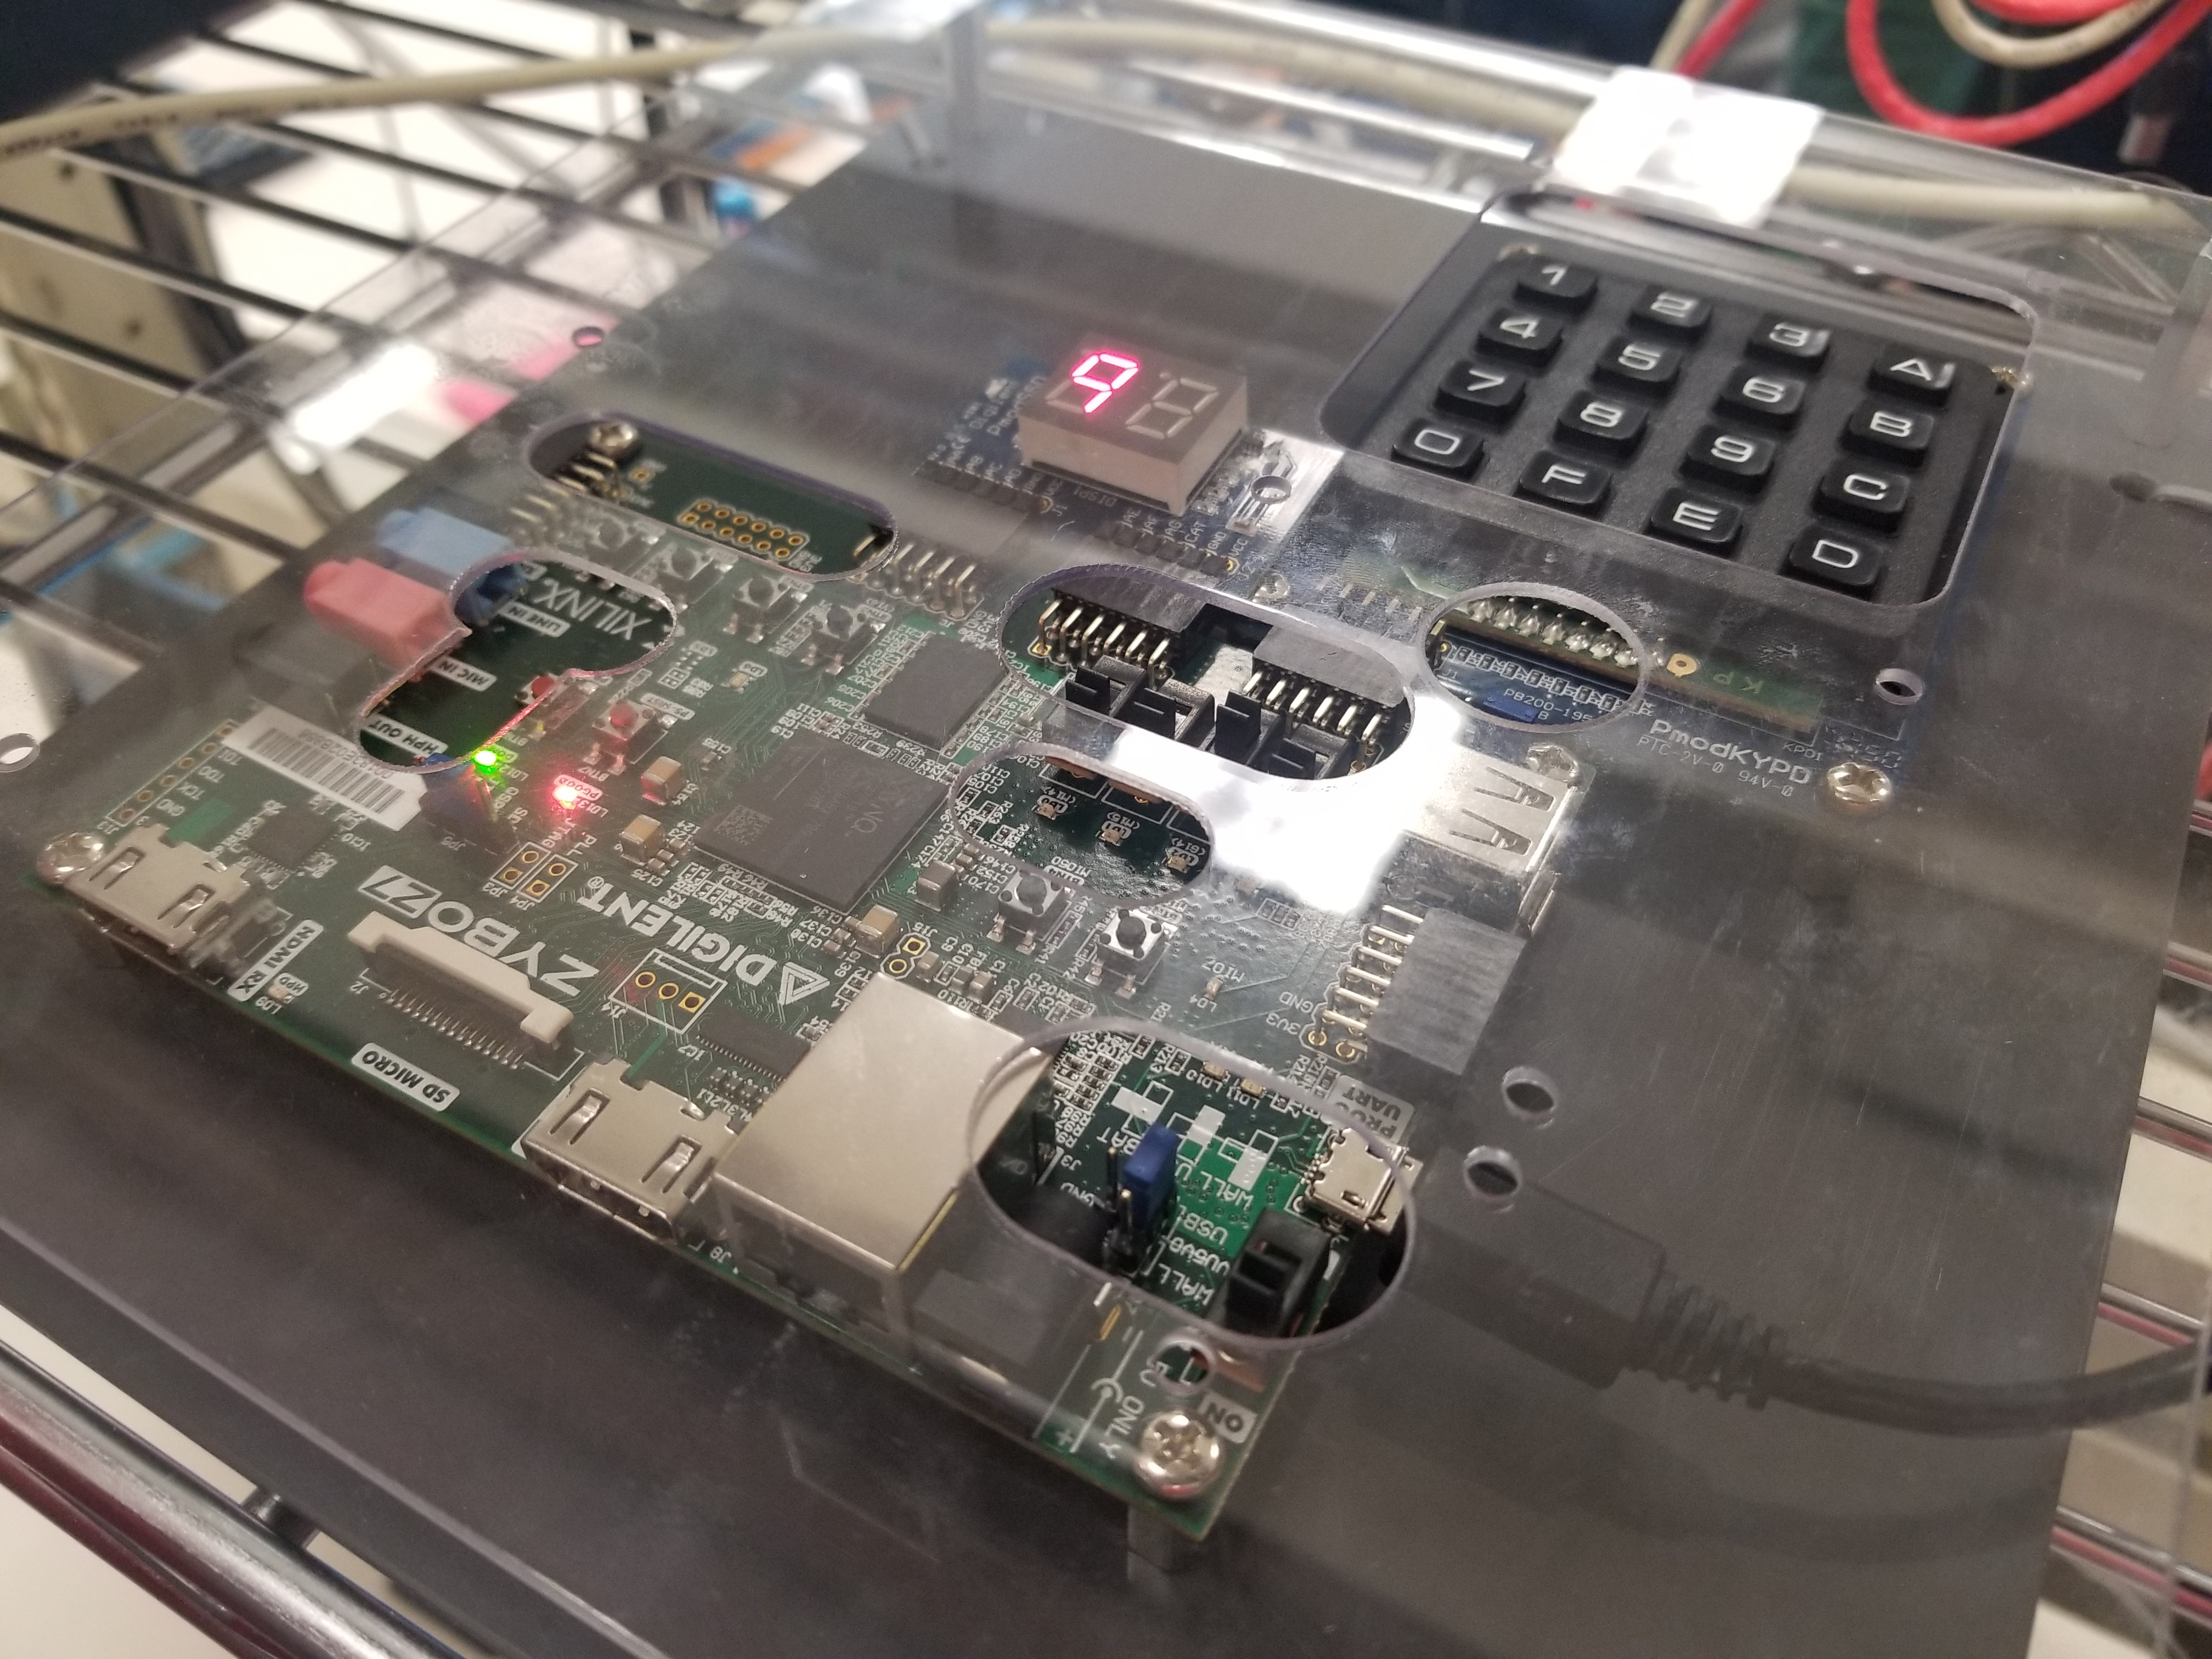
\includegraphics[width=125mm]{display_single.jpg}
        \caption{Single-character hexadecimal deisplay.}
        \label{fig:display_single}
    \end{figure}

    
    \begin{figure}[H]
        % Mess around with widths later
        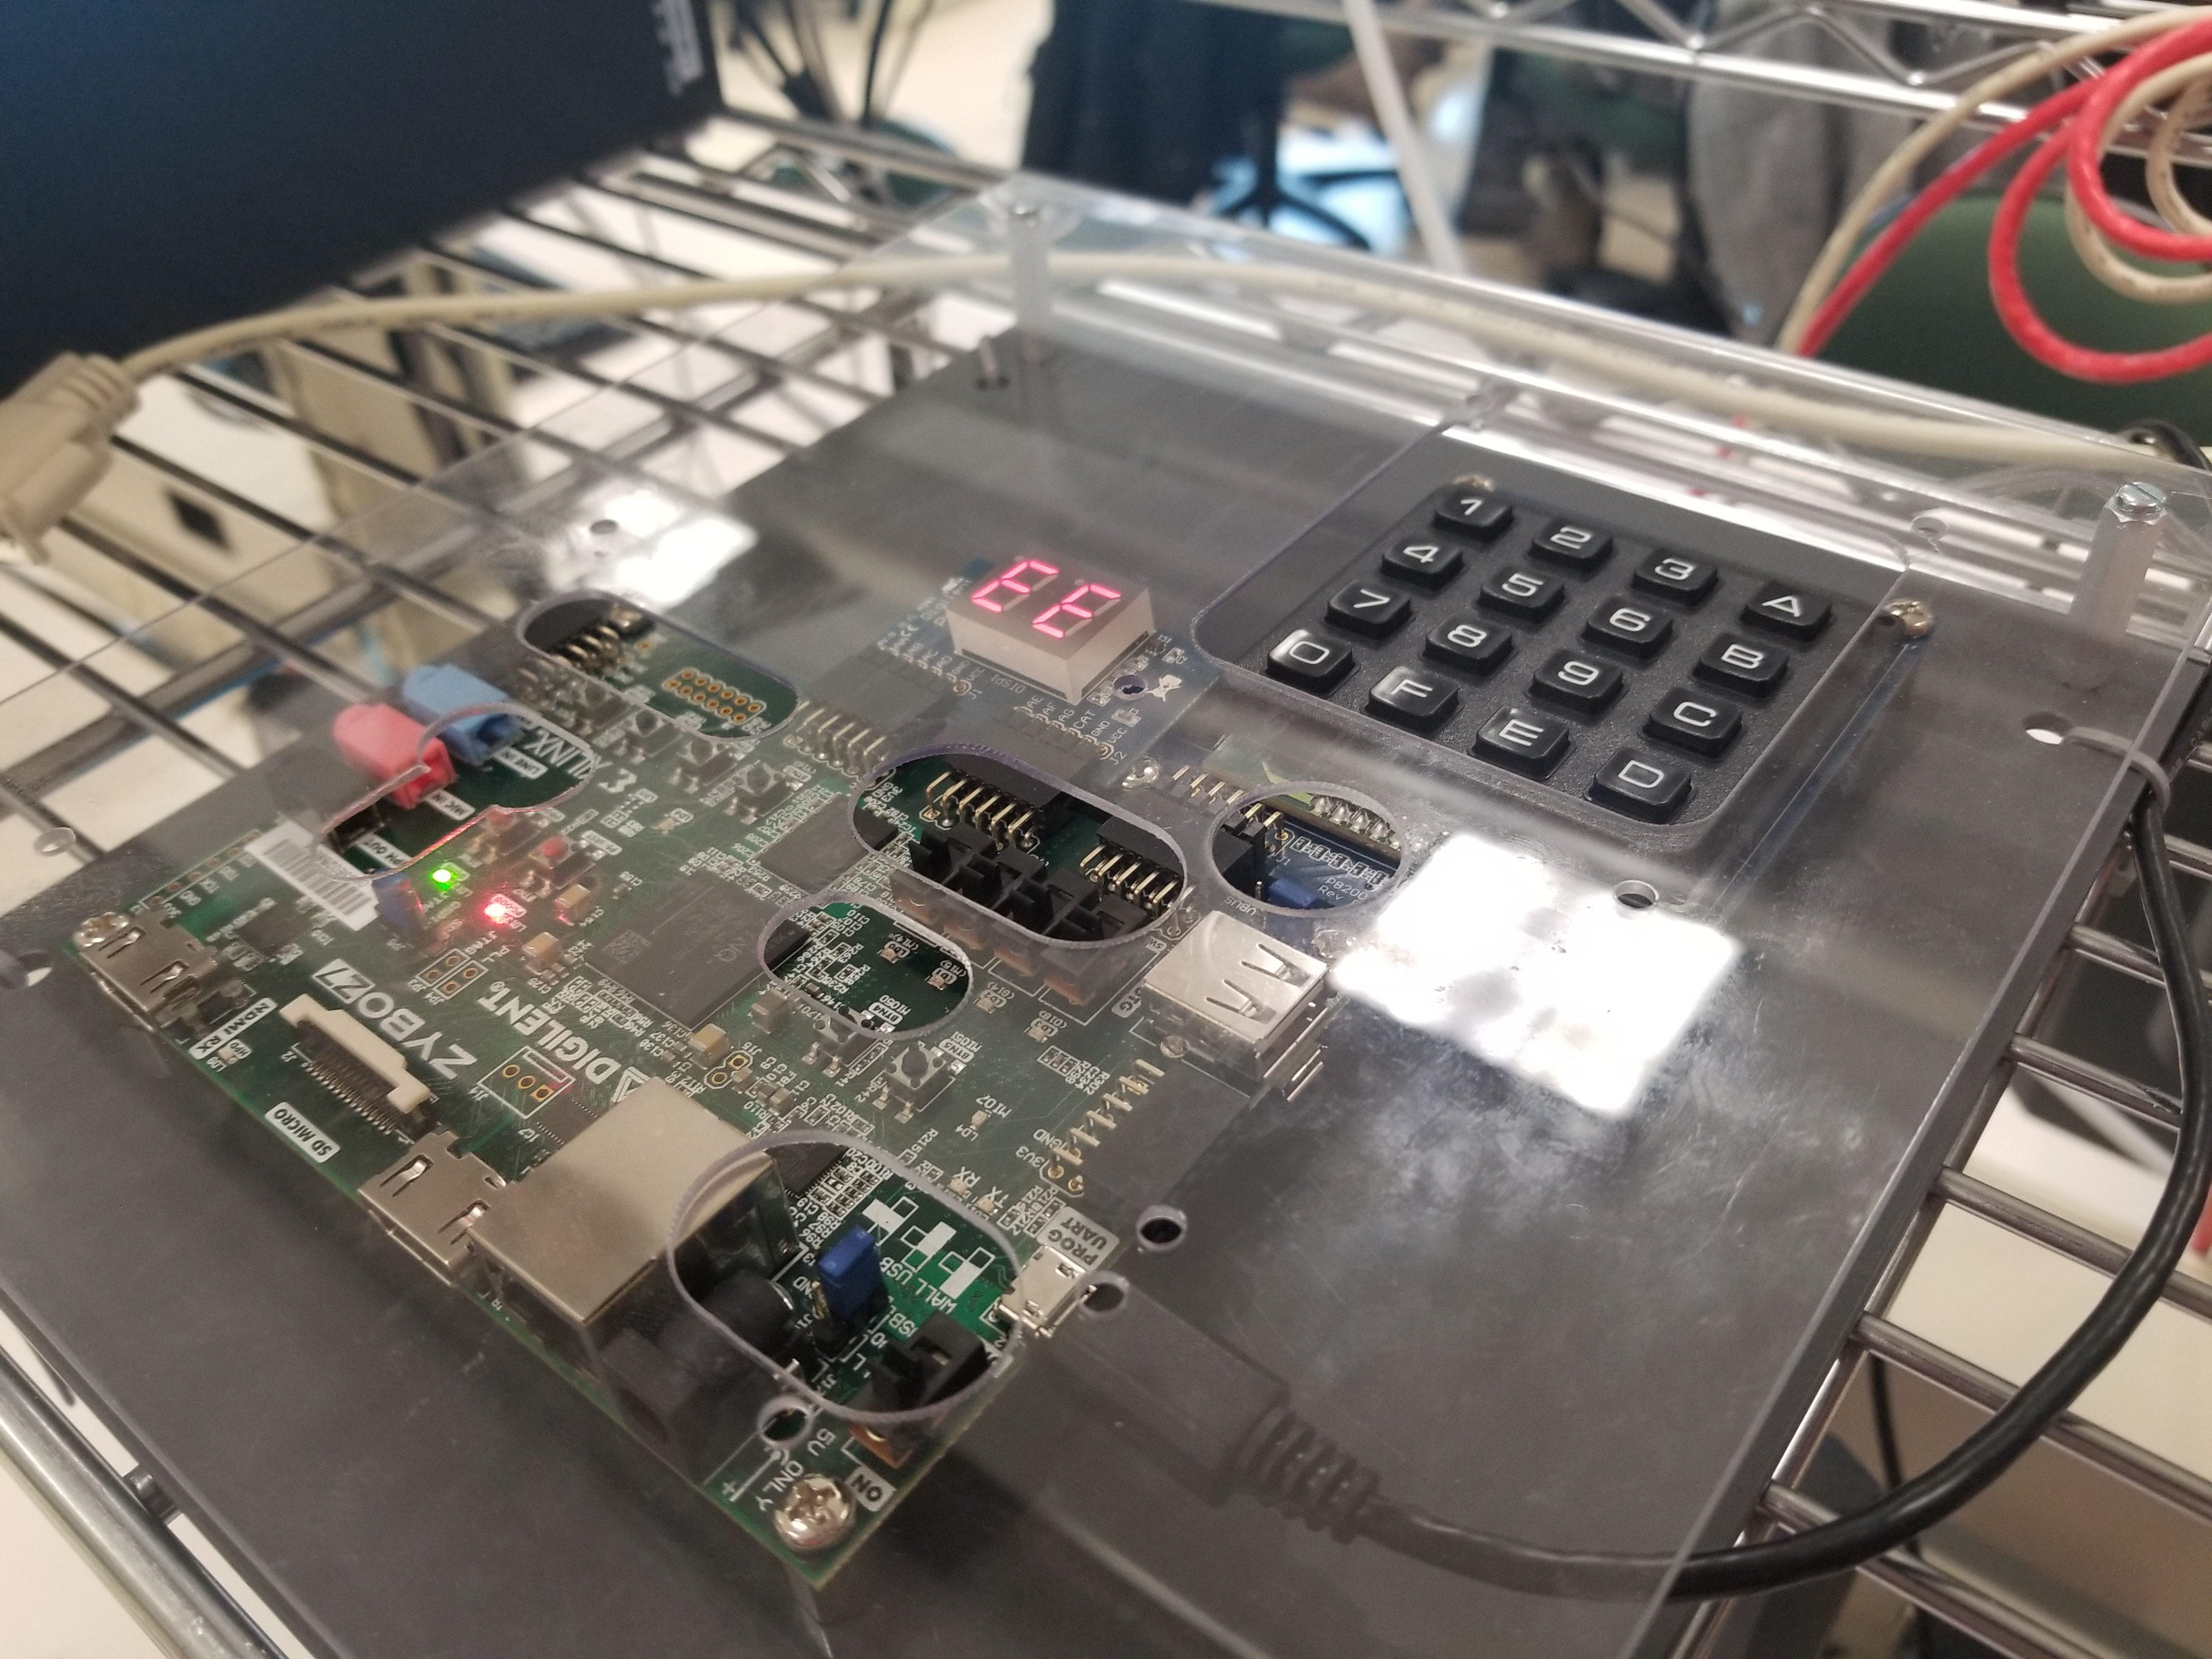
\includegraphics[width=125mm]{counter_dual.jpg}
        \caption{Dual character upcounter.}
        \label{fig:counter_dual}
    \end{figure}


\end{document}
